%----------------------------------------------------------------------------------------
%	PACKAGES AND THEMES
%----------------------------------------------------------------------------------------
\documentclass[aspectratio=169,xcolor=dvipsnames]{beamer}
\usetheme{SimplePlus}
\setbeamertemplate{footline}[frame number]{}

\usepackage{hyperref}
\usepackage{graphicx} % Allows including images
\usepackage{booktabs} % Allows the use of \toprule, \midrule and \bottomrule in tables
\usepackage{siunitx}
\usepackage{import}
\usepackage{amsmath}
%\numberwithin{equation}{section}% numera eq come #section.#formula
\usepackage{amsthm}
\usepackage{stmaryrd}
\usepackage{amssymb}
\usepackage{wasysym}
\usepackage{cancel}
\usepackage{textcomp}
\usepackage{subcaption}
\definecolor{myred}{rgb}{0.545, 0.172, 0.031}
\DeclareUnicodeCharacter{25CF}{\lgblkcircle}
%\usepackage{cleveref}
%----------------------------------------------------------------------------------------
%	TITLE PAGE
%----------------------------------------------------------------------------------------

\title[short title]{Modelli numerici elasto-plastici} % The short title appears at the bottom of every slide, the full title is only on the title page
\subtitle{Hardening isotropo e cinematico}

\author[Pin-Yen] {Alessandro Mastrofini}

\institute[NTU] % Your institution as it will appear on the bottom of every slide, may be shorthand to save space
{
Meccanica Computazionale dei Tessuti e Biomateriali \\
Università degli Studi di Roma Tor Vergata% Your institution for the title page
}
\date{2022} % Date, can be changed to a custom date

\graphicspath{{figures/}} %Setting the graphicspat%h
\graphicspath{{figures/}} %Setting the graphicspath
\makeatletter
\providecommand*{\input@path}{}
\edef\input@path{{figures/}{}\input@path}% prepend
\makeatother
%----------------------------------------------------------------------------------------
%	PRESENTATION SLIDES
%----------------------------------------------------------------------------------------

\begin{document}

\begin{frame}
    % Print the title page as the first slide
    \titlepage
\end{frame}

%------------------------------------------------
\section{First Section}
%------------------------------------------------
\begin{frame}{Structural behaviour}
	\begin{figure}
		\begin{minipage}[c]{0.3\linewidth}
			\tiny{
\def\svgwidth{\linewidth}
\input{isotropic.pdf_tex}}
		\end{minipage}\hfill
	\begin{minipage}[c]{0.3\linewidth}
		\tiny{
\def\svgwidth{\linewidth}
\input{kinematic.pdf_tex}}
	\end{minipage}\hfill
\begin{minipage}{0.3\linewidth}
	\centering
	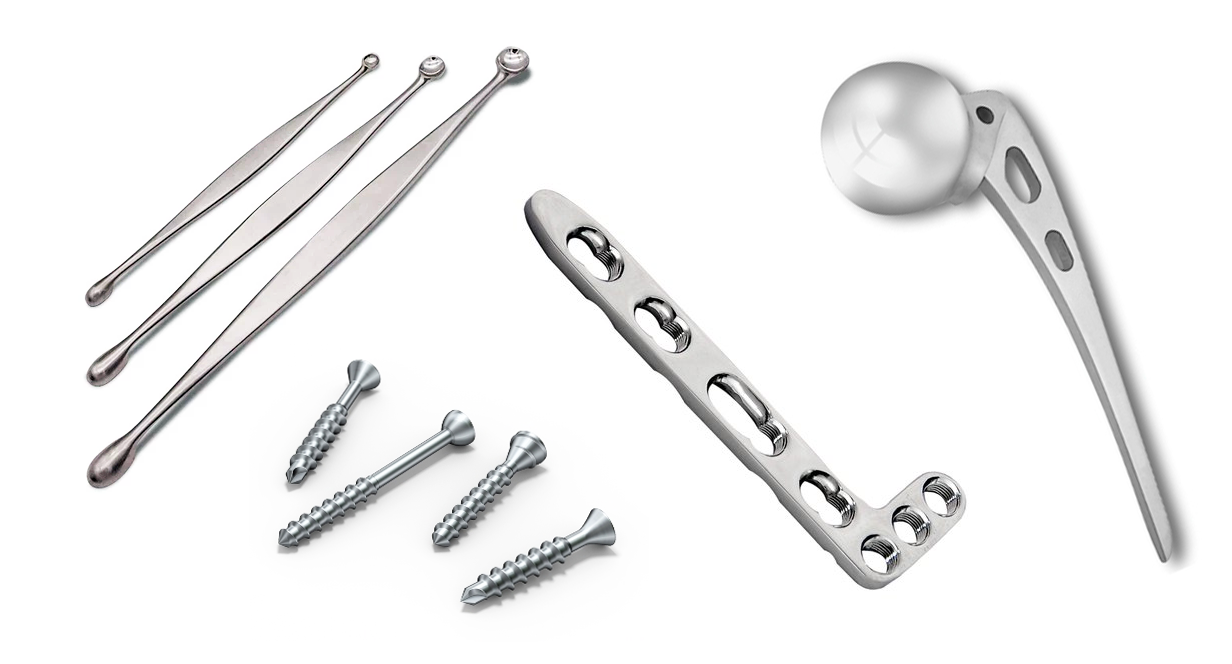
\includegraphics[width=\linewidth]{stainless_steell_biomedical.png}
\vfill
\vspace{0.2\linewidth}
	\tiny{
\begin{tabular}{c|c|c}

	$\sigma_y$ (MPa)& $\sigma_u$ (MPa)& $\varepsilon_u$ (\%) \\
	\hline
	175 &  500& 45 \\
	\hline
	190 & 600 & 45 \\
	\hline
	280& 680 & 35 \\
	\hline
	450& 700 & 25 \\
	\hline
	345&  517& 25 \\
	\hline
	276& 517 &30  \\
	\hline
	414& 274 & 20 \\
	\hline
	276& 759 &60  \\

\end{tabular}}\vfill
\end{minipage}\hfill

		\end{figure}
\end{frame}

\begin{frame}{Patch test}
 	\begin{figure}
 	\begin{minipage}[c]{0.2\linewidth}
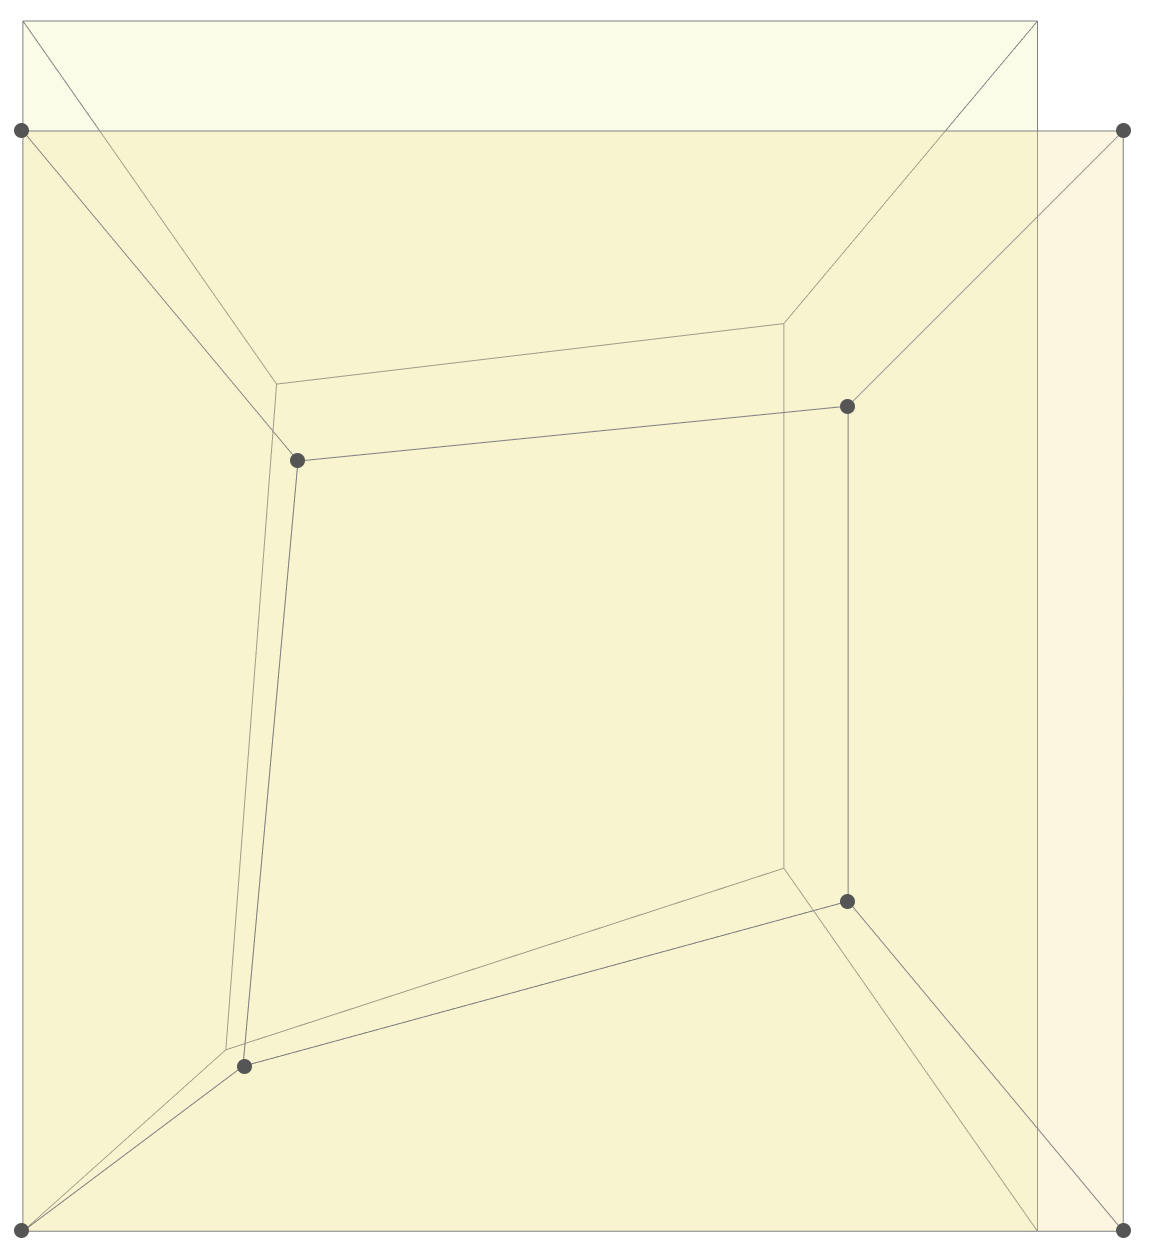
\includegraphics[width=0.9\linewidth]{patch_def.png}
 	\end{minipage}\hfill
 	\begin{minipage}[c]{0.8\linewidth}
 		\begin{minipage}{0.32\linewidth}
 			    \fontsize{3pt}{4pt}\selectfont{
 			\def\svgwidth{\linewidth}
 			\input{patch_175_1054_tex.pdf_tex}}
 		\end{minipage}\hfill
 		\begin{minipage}{0.32\linewidth}
 		    \fontsize{3pt}{4pt}\selectfont{
 			\def\svgwidth{\linewidth}
 			\input{patch_375_1054_tex.pdf_tex}}
 	\end{minipage}\hfill	\begin{minipage}{0.32\linewidth}
 	    \fontsize{3pt}{4pt}\selectfont{
 		\def\svgwidth{\linewidth}
 		\input{patch_425_1054_tex.pdf_tex}}
 \end{minipage}\hfill
 	\end{minipage}\hfill
\end{figure}
%%%%%
\begin{figure}
 \begin{minipage}{\linewidth}
  	\begin{minipage}[c]{0.3\linewidth}
 	 \fontsize{3pt}{4pt}\selectfont{
 		\def\svgwidth{\linewidth}
 		\input{patch_sigma_vs_harden_tex.pdf_tex}}
 \end{minipage}\hfill
  	\begin{minipage}[c]{0.34\linewidth}
	 \fontsize{3pt}{4pt}\selectfont{
		\def\svgwidth{\linewidth}
		\input{patch_sigma_vs_sigmay_tex.pdf_tex}}
\end{minipage}\hfill
  	\begin{minipage}[c]{0.32\linewidth}
	 \fontsize{3pt}{4pt}\selectfont{
		\def\svgwidth{\linewidth}
		\input{patch_contour.pdf_tex}}
\end{minipage}\hfill
%%%%%%%%%%%%%%%%%
 \end{minipage}
\end{figure}
 
\end{frame}

\begin{frame}{Crack plate}
	
	\begin{figure}
		\begin{minipage}{\linewidth}
			\begin{minipage}[c]{0.3\linewidth}
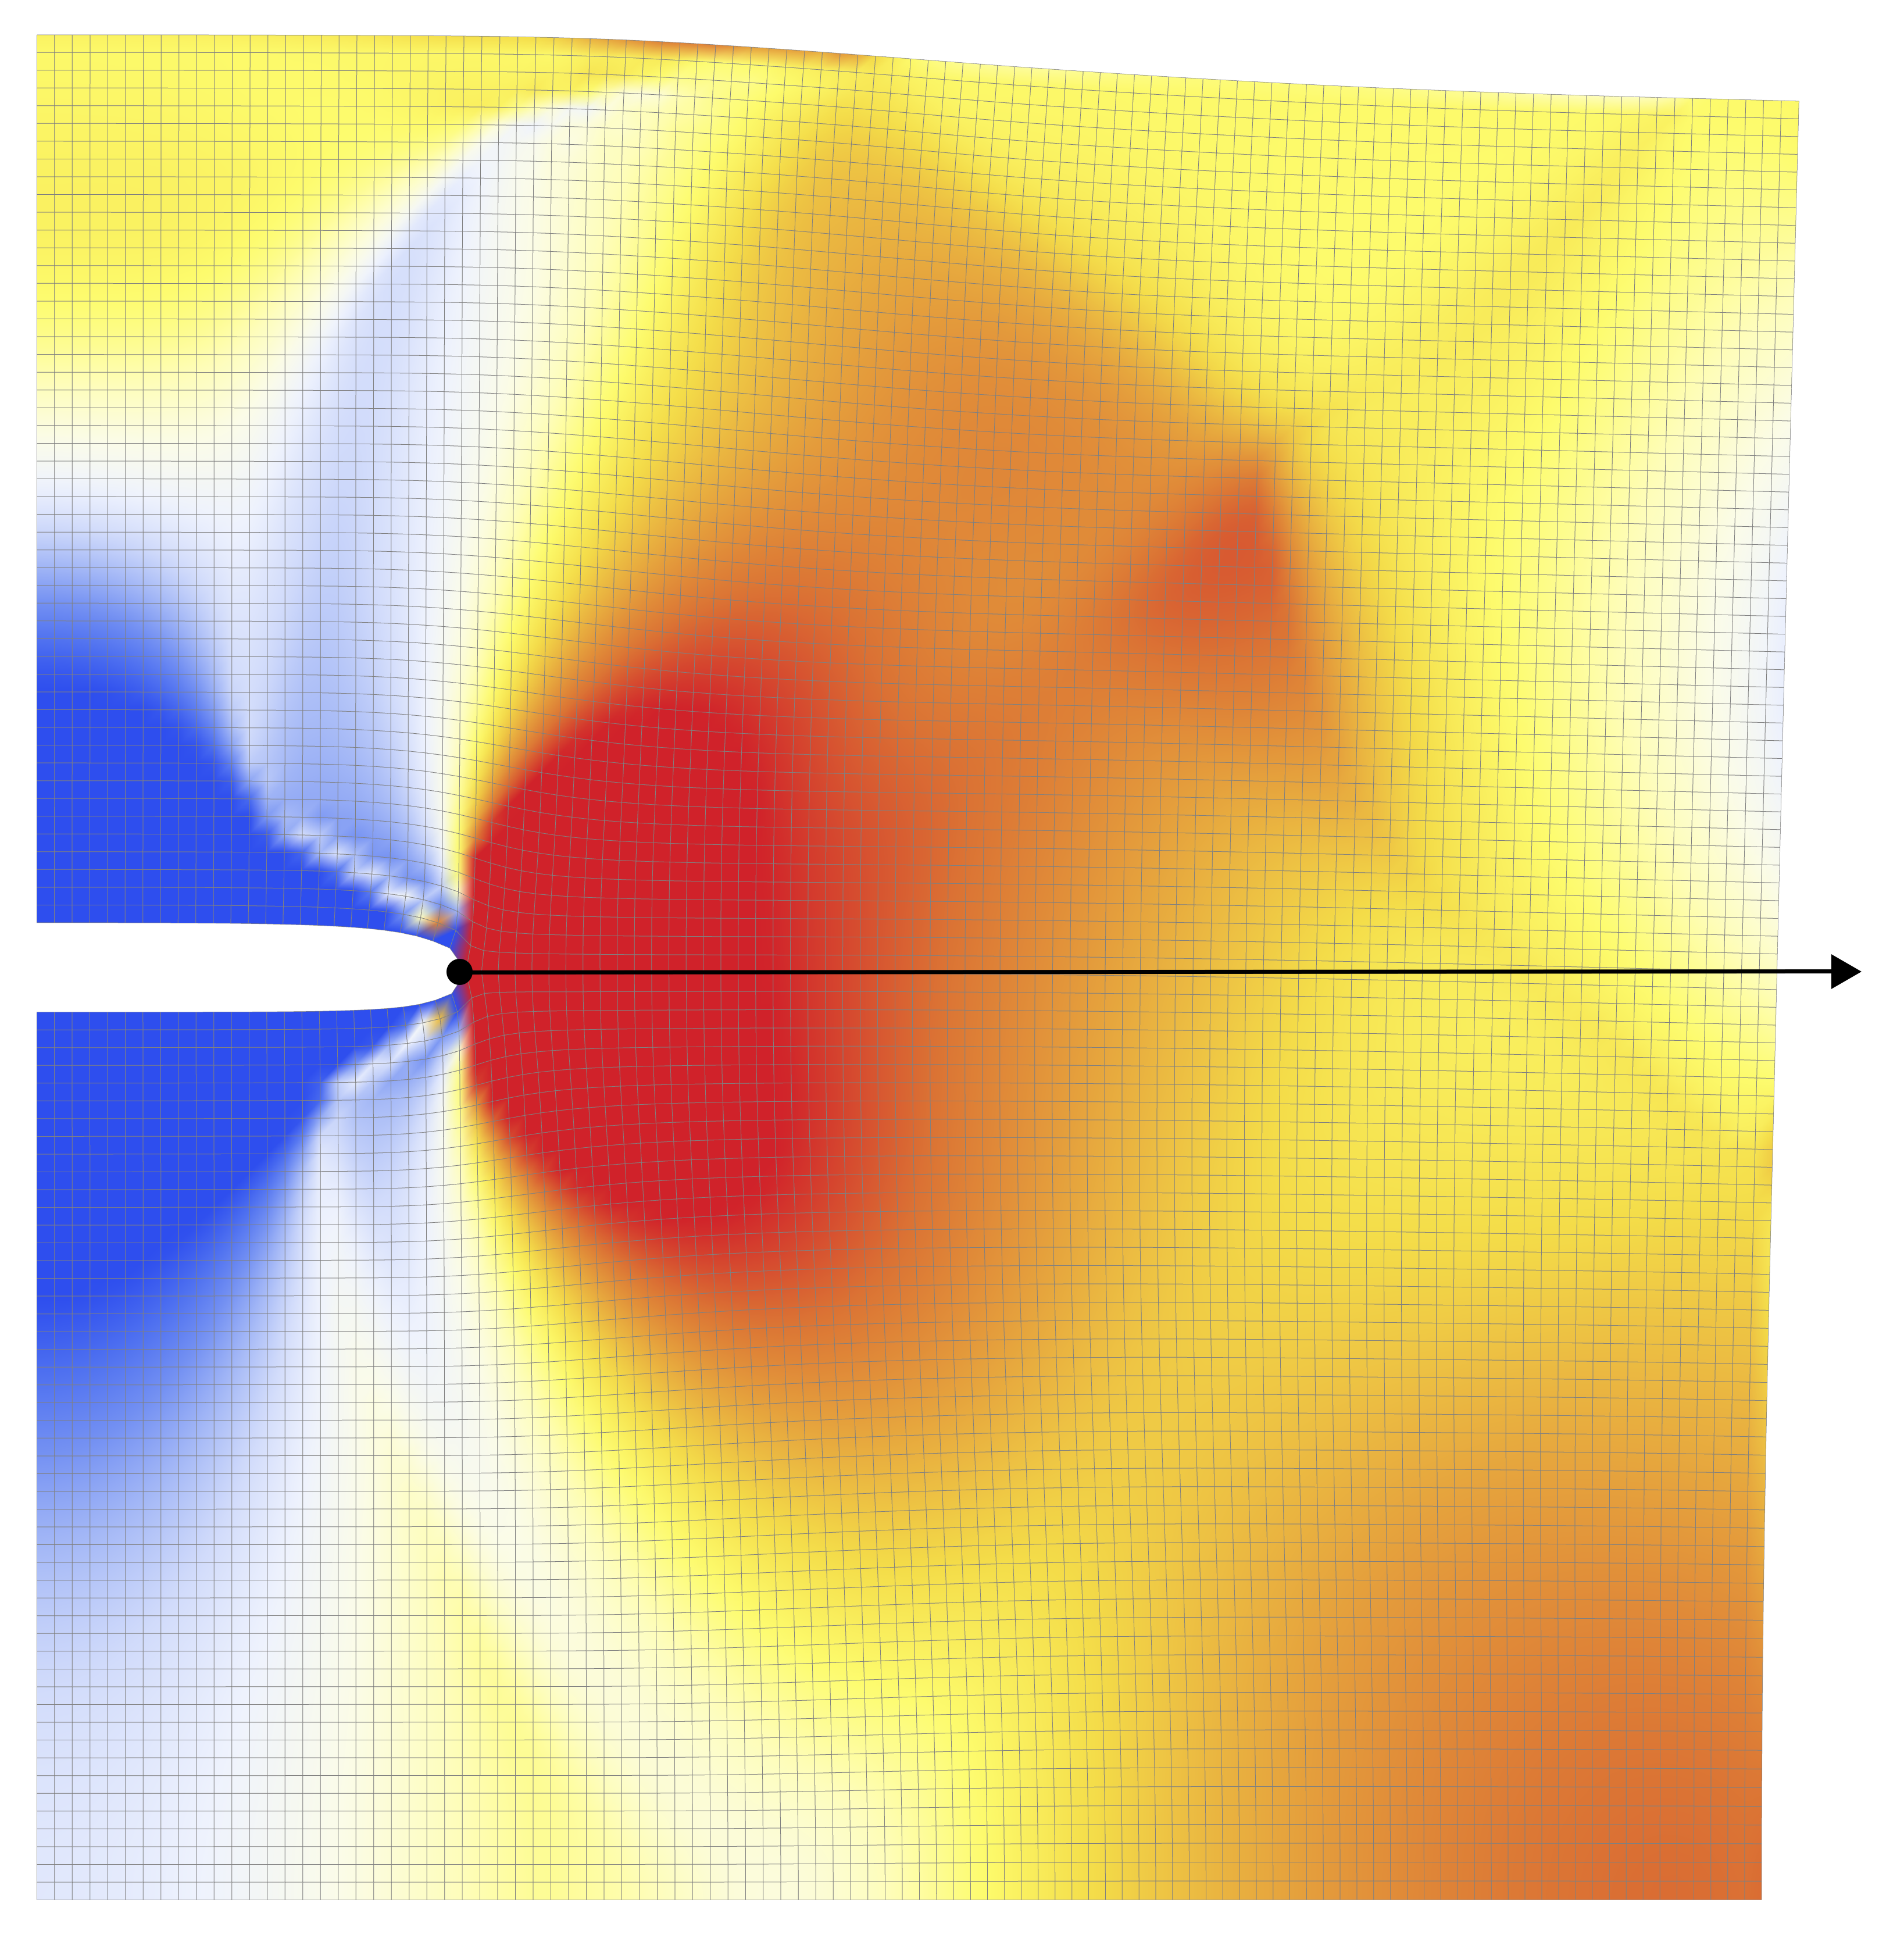
\includegraphics[width=\linewidth]{plate_def.png}
			\end{minipage}\hfill
		\begin{minipage}{0.65\linewidth}
		\begin{minipage}[b]{0.3\linewidth}
		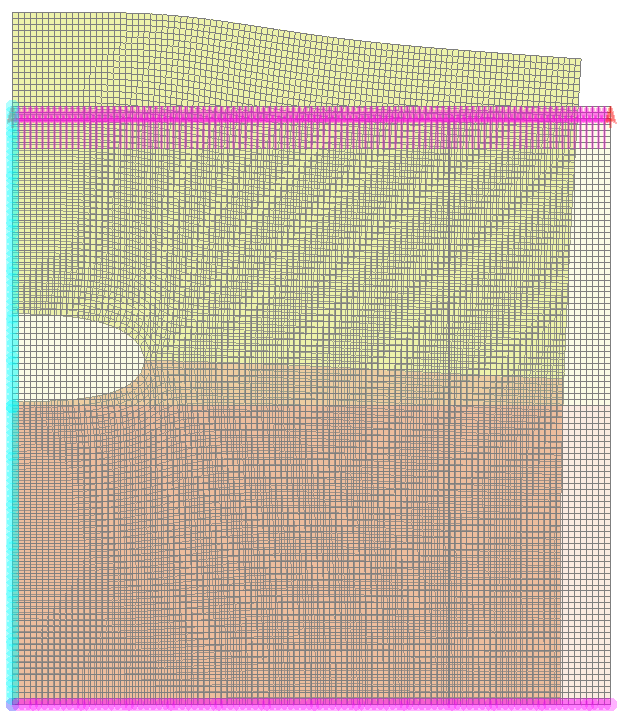
\includegraphics[width=\linewidth]{plate_175_1145.pdf}
						\centering
					 \fontsize{3pt}{4pt}\selectfont{
			$\sigma_y=175\text { MPa}$\\$H=1145\text { MPa}$}
	\end{minipage}\hfill
			\begin{minipage}[b]{0.3\linewidth}
				\centering
					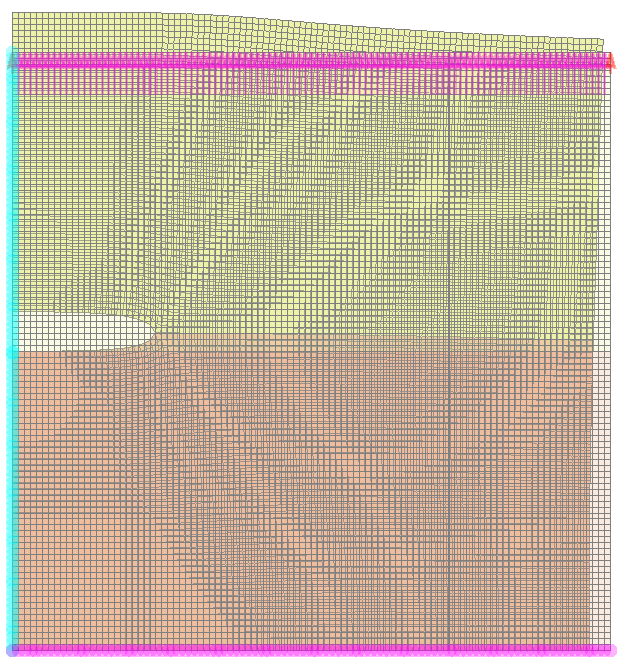
\includegraphics[width=\linewidth]{plate_250_1509.pdf}
								 \fontsize{3pt}{4pt}\selectfont{
						$\sigma_y=250\text { MPa}$\\$H=1509\text { MPa}$}
			\end{minipage}\hfill
			\begin{minipage}[b]{0.3\linewidth}
								\centering
				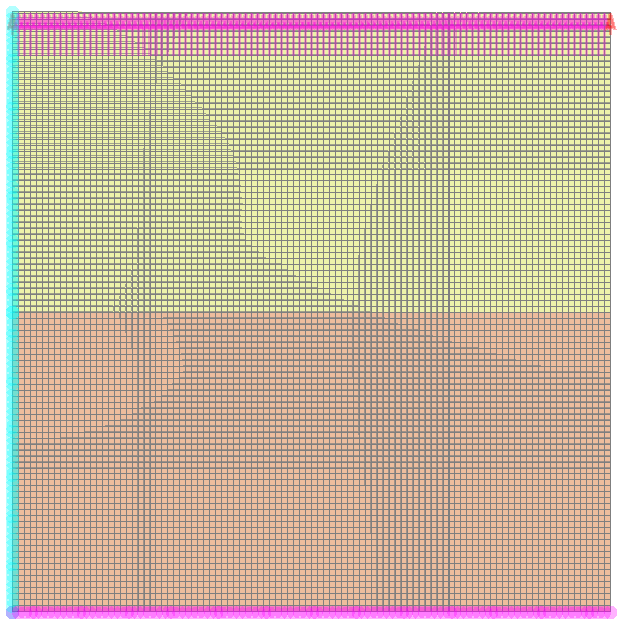
\includegraphics[width=\linewidth]{plate_425_1054.pdf}
					 \fontsize{3pt}{4pt}\selectfont{
					$\sigma_y=425\text { MPa}$\\$H=1054\text { MPa}$}
			\end{minipage}\hfill
			%%%%%%%%%%%%%%%%%
		\end{minipage}
\end{minipage}
%\pause
\begin{minipage}{\linewidth}
	\centering
		\begin{minipage}[c]{0.25\linewidth}
 \fontsize{3pt}{4pt}\selectfont{
	\def\svgwidth{\linewidth}
	\input{sigmayy_vs_s_tex.pdf_tex}}
	\end{minipage}\hfill
	\begin{minipage}[c]{0.26\linewidth}
	\fontsize{3pt}{4pt}\selectfont{
		\def\svgwidth{\linewidth}
		\input{plate_contour.pdf_tex}}
\end{minipage}\hfill
	\begin{minipage}[c]{0.22\linewidth}
	 \fontsize{3pt}{4pt}\selectfont{
		\def\svgwidth{\linewidth}
		\input{plate_v_vs_harden_tex.pdf_tex}}
	\end{minipage}\hfill
	\begin{minipage}[c]{0.27\linewidth}
	 \fontsize{3pt}{4pt}\selectfont{
	\def\svgwidth{\linewidth}
	\input{plate_v_vs_sigmay_tex.pdf_tex}}
\end{minipage}\hfill
	\end{minipage}
	\end{figure}

\end{frame}

\begin{frame}{Stress intensity factor}
	\begin{figure}
	\begin{minipage}{0.35\linewidth}
		\begin{minipage}[c]{0.5\linewidth}
	 \fontsize{3pt}{4pt}\selectfont{
	\def\svgwidth{\linewidth}
	\input{sigmayy_L8_tex.pdf_tex}}
		\end{minipage}\hfill
		\begin{minipage}[c]{0.5\linewidth}
	 \fontsize{3pt}{4pt}\selectfont{
	\def\svgwidth{\linewidth}
	\input{sigmayy_L4_tex.pdf_tex}}
		\end{minipage}\hfill
		\begin{minipage}[c]{0.5\linewidth}
 \fontsize{3pt}{4pt}\selectfont{
	\def\svgwidth{\linewidth}
	\input{K_L8_tex.pdf_tex}}
	\end{minipage}\hfill
	\begin{minipage}[c]{0.5\linewidth}
 \fontsize{3pt}{4pt}\selectfont{
	\def\svgwidth{\linewidth}
	\input{K_L4_tex.pdf_tex}}
	\end{minipage}\hfill

		\begin{minipage}[c]{0.5\linewidth}
	 \fontsize{3pt}{4pt}\selectfont{
	\def\svgwidth{\linewidth}
	\input{sigmayy_L2_tex.pdf_tex}}
		\end{minipage}\hfill
		\begin{minipage}[c]{0.5\linewidth}
	 \fontsize{3pt}{4pt}\selectfont{
	\def\svgwidth{\linewidth}
	\input{sigmayy_3L4_tex.pdf_tex}}
		\end{minipage}\hfill
		\begin{minipage}[c]{0.5\linewidth}
 \fontsize{3pt}{4pt}\selectfont{
	\def\svgwidth{\linewidth}
	\input{K_L2_tex.pdf_tex}}
	\end{minipage}\hfill
	\begin{minipage}[c]{0.5\linewidth}
 \fontsize{3pt}{4pt}\selectfont{
	\def\svgwidth{\linewidth}
	\input{K_3L4_tex.pdf_tex}}
	\end{minipage}\hfill
	\end{minipage}
	\begin{minipage}{0.6\linewidth}
		\centering
		\begin{center}
		\footnotesize{\begin{equation*}
			K={\sigma_y\over q}
		\end{equation*}}
	\hspace{0.15\linewidth} \fontsize{5pt}{4pt}\selectfont{
		\def\svgwidth{0.9\linewidth}
		\input{K_tex.pdf_tex}}
			\end{center}
\end{minipage}
%%%%%%%%%%%%%%%%%
\end{figure}
\end{frame}

\begin{frame}{Isotropic and kinematic hardening}
		\begin{figure}
		\begin{minipage}{0.35\linewidth}
			\centering
			\tiny{Patch test}\\
			\begin{minipage}[c]{0.5\linewidth}
\fontsize{3pt}{4pt}\selectfont{
	\def\svgwidth{\linewidth}
	\input{patch_isotropic_tex.pdf_tex}}
			\end{minipage}\hfill
			\begin{minipage}[c]{0.5\linewidth}
\fontsize{3pt}{4pt}\selectfont{
	\def\svgwidth{\linewidth}
	\input{patch_kinematic_tex.pdf_tex}}
			\end{minipage}\hfill
		\begin{minipage}{\linewidth}
			\centering
				\vspace{0.05\linewidth}	\tiny{Load}
\fontsize{3pt}{4pt}\selectfont{
	\def\svgwidth{0.9\linewidth}
	\input{load_tex.pdf_tex}}
		\end{minipage}\hfill		
	\vspace{0.05\linewidth}	\tiny{Plate\\}
			\begin{minipage}{0.5\linewidth}
			\centering
\fontsize{3pt}{4pt}\selectfont{
	\def\svgwidth{0.8\linewidth}
	\input{plate_isotropic_tex.pdf_tex}}
		\end{minipage}\hfill
		\begin{minipage}{0.5\linewidth}
			\centering
\fontsize{3pt}{4pt}\selectfont{
	\def\svgwidth{0.9\linewidth}
	\input{plate_kinematic_tex.pdf_tex}}
		\end{minipage}\hfill
		\end{minipage}
		\begin{minipage}{0.6\linewidth}
			\centering
			\tiny{Cook's membrane\\}
						\begin{minipage}{0.5\linewidth}
				\centering
				\fontsize{3pt}{4pt}\selectfont{
					\def\svgwidth{0.9\linewidth}
					\input{cook_isotropic_tex.pdf_tex}}
			\end{minipage}\hfill
			\begin{minipage}{0.5\linewidth}
				\centering
				\fontsize{3pt}{4pt}\selectfont{
					\def\svgwidth{\linewidth}
					\input{cook_kinematic_tex.pdf_tex}}
			\end{minipage}\hfill
		%%%%%%%%%%%%%%%%%%%%%
			\begin{minipage}{0.5\linewidth}
				\centering
	\fontsize{4pt}{4pt}\selectfont{isotropic hardening\\}
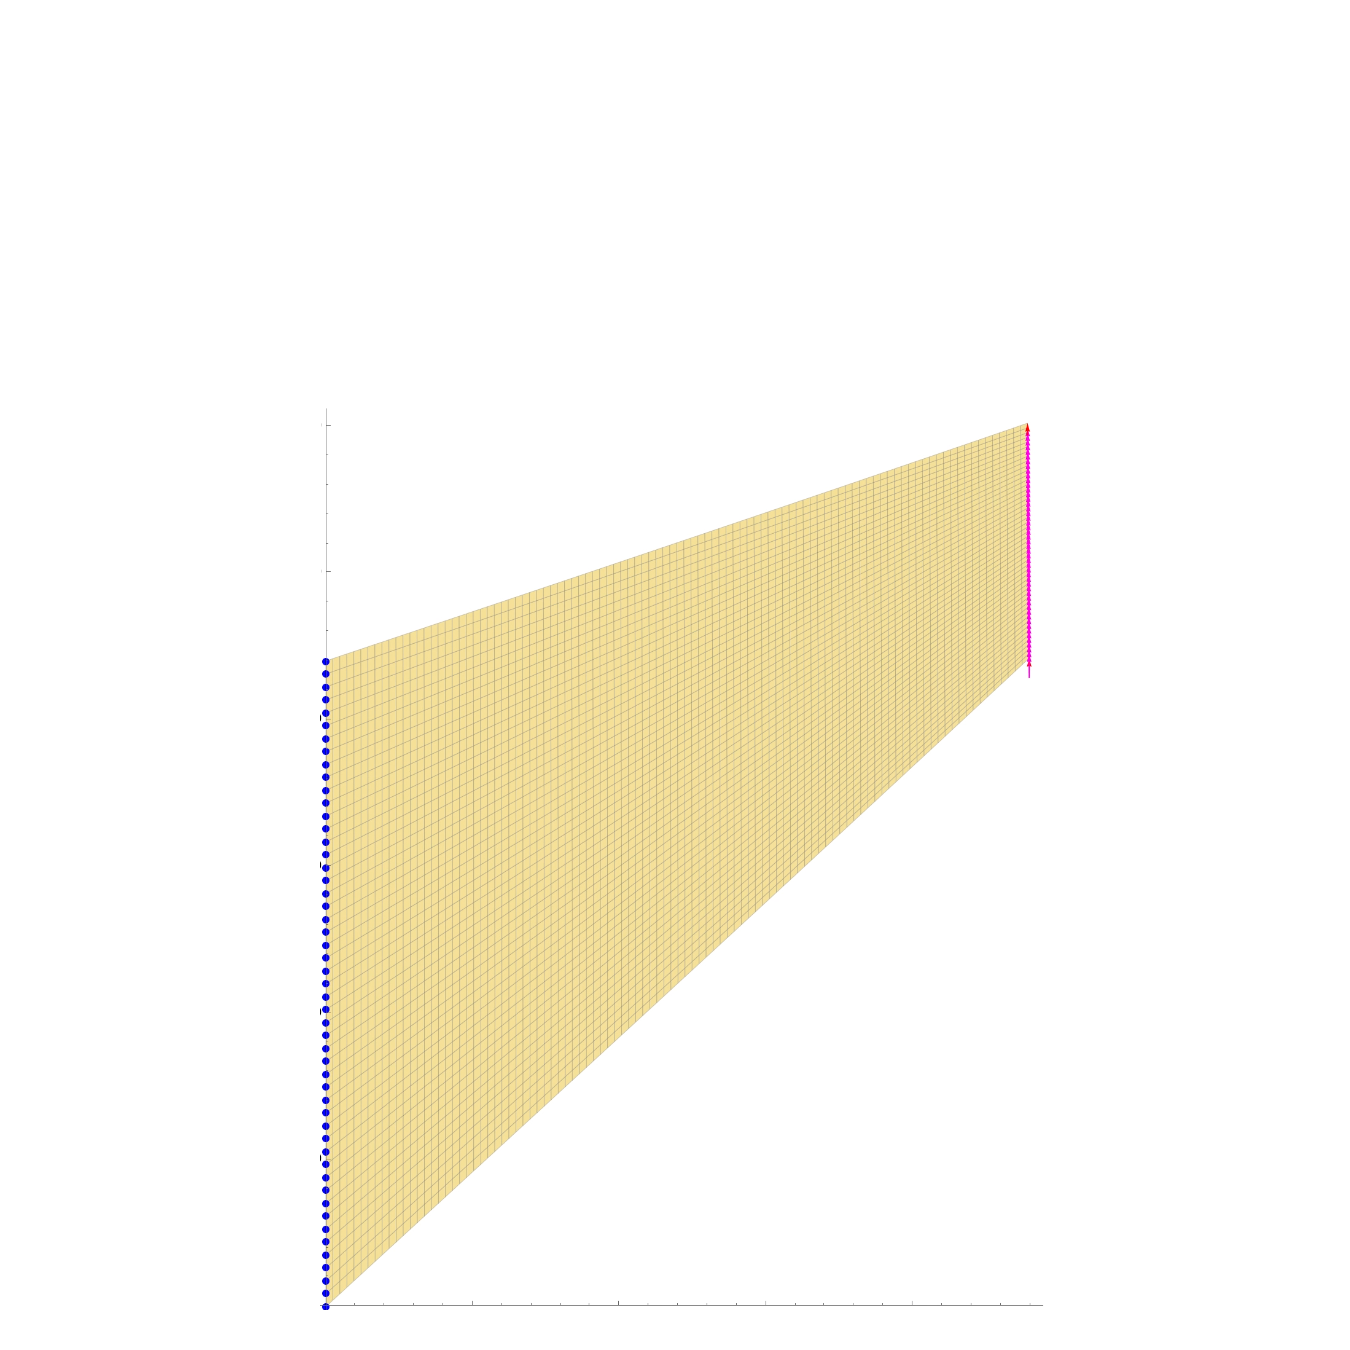
\includegraphics[width=0.3\linewidth]{iso1.png}\hfill
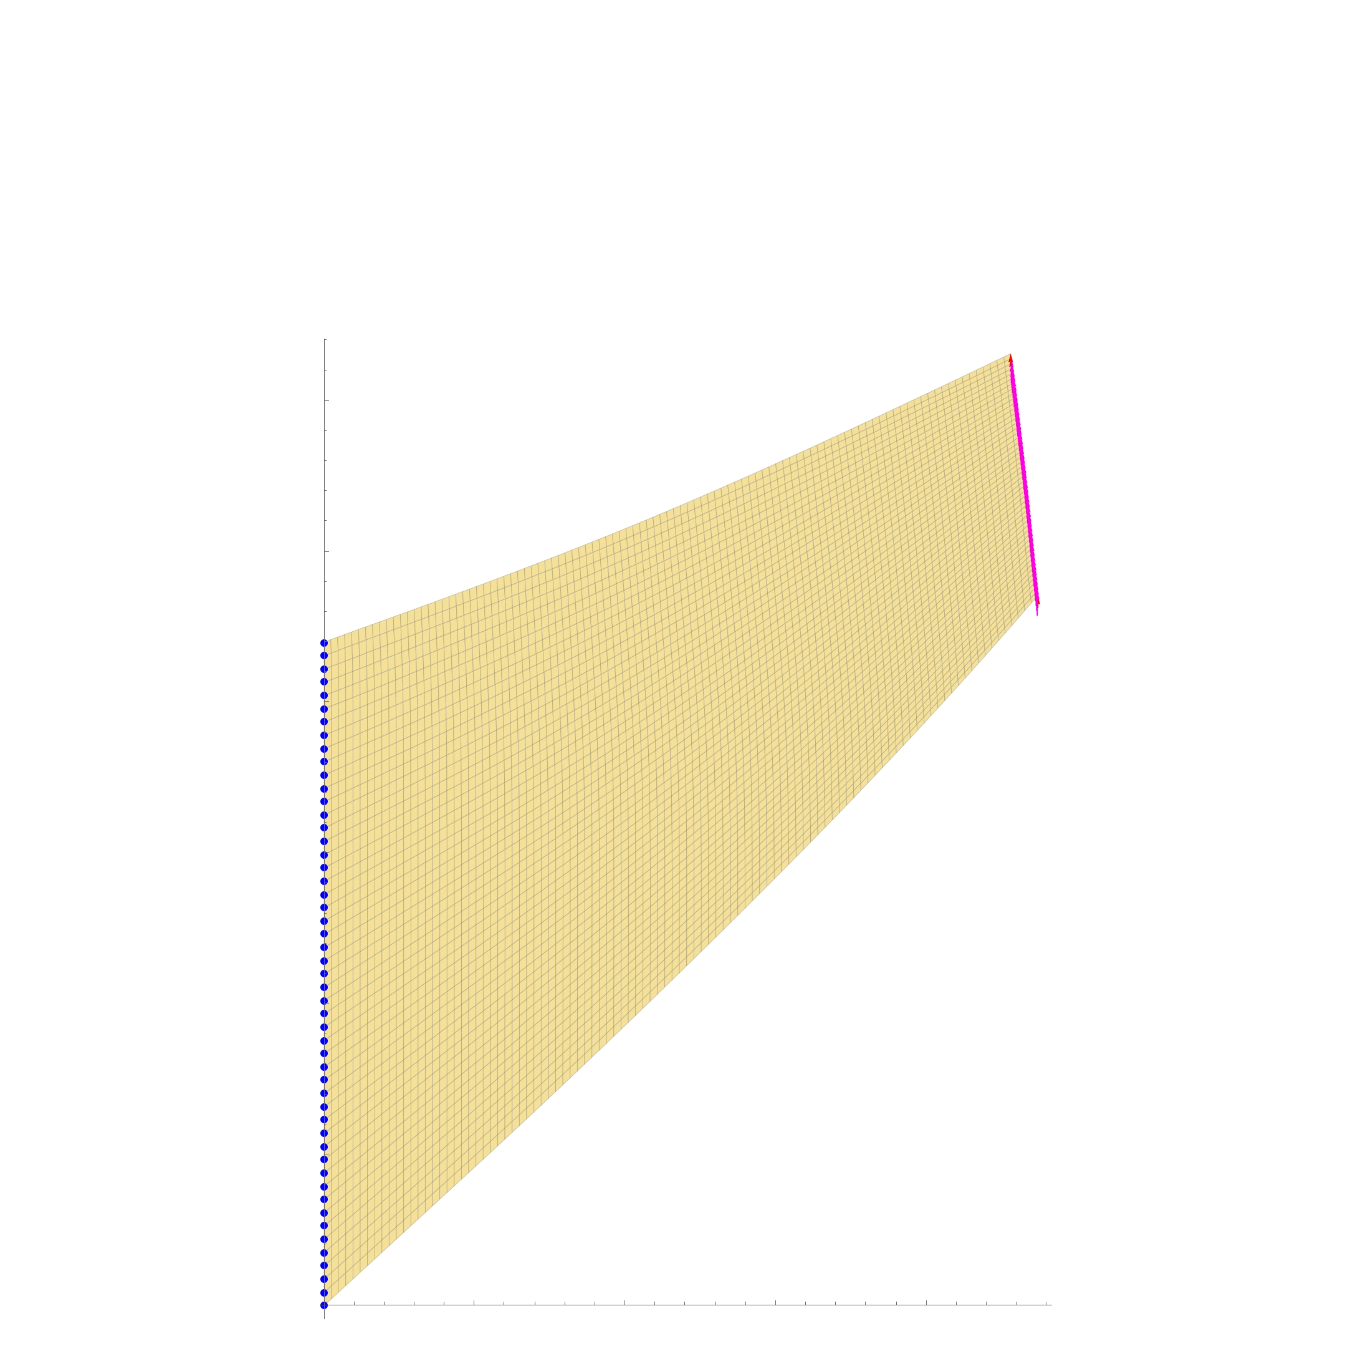
\includegraphics[width=0.3\linewidth]{iso2.png}\hfill
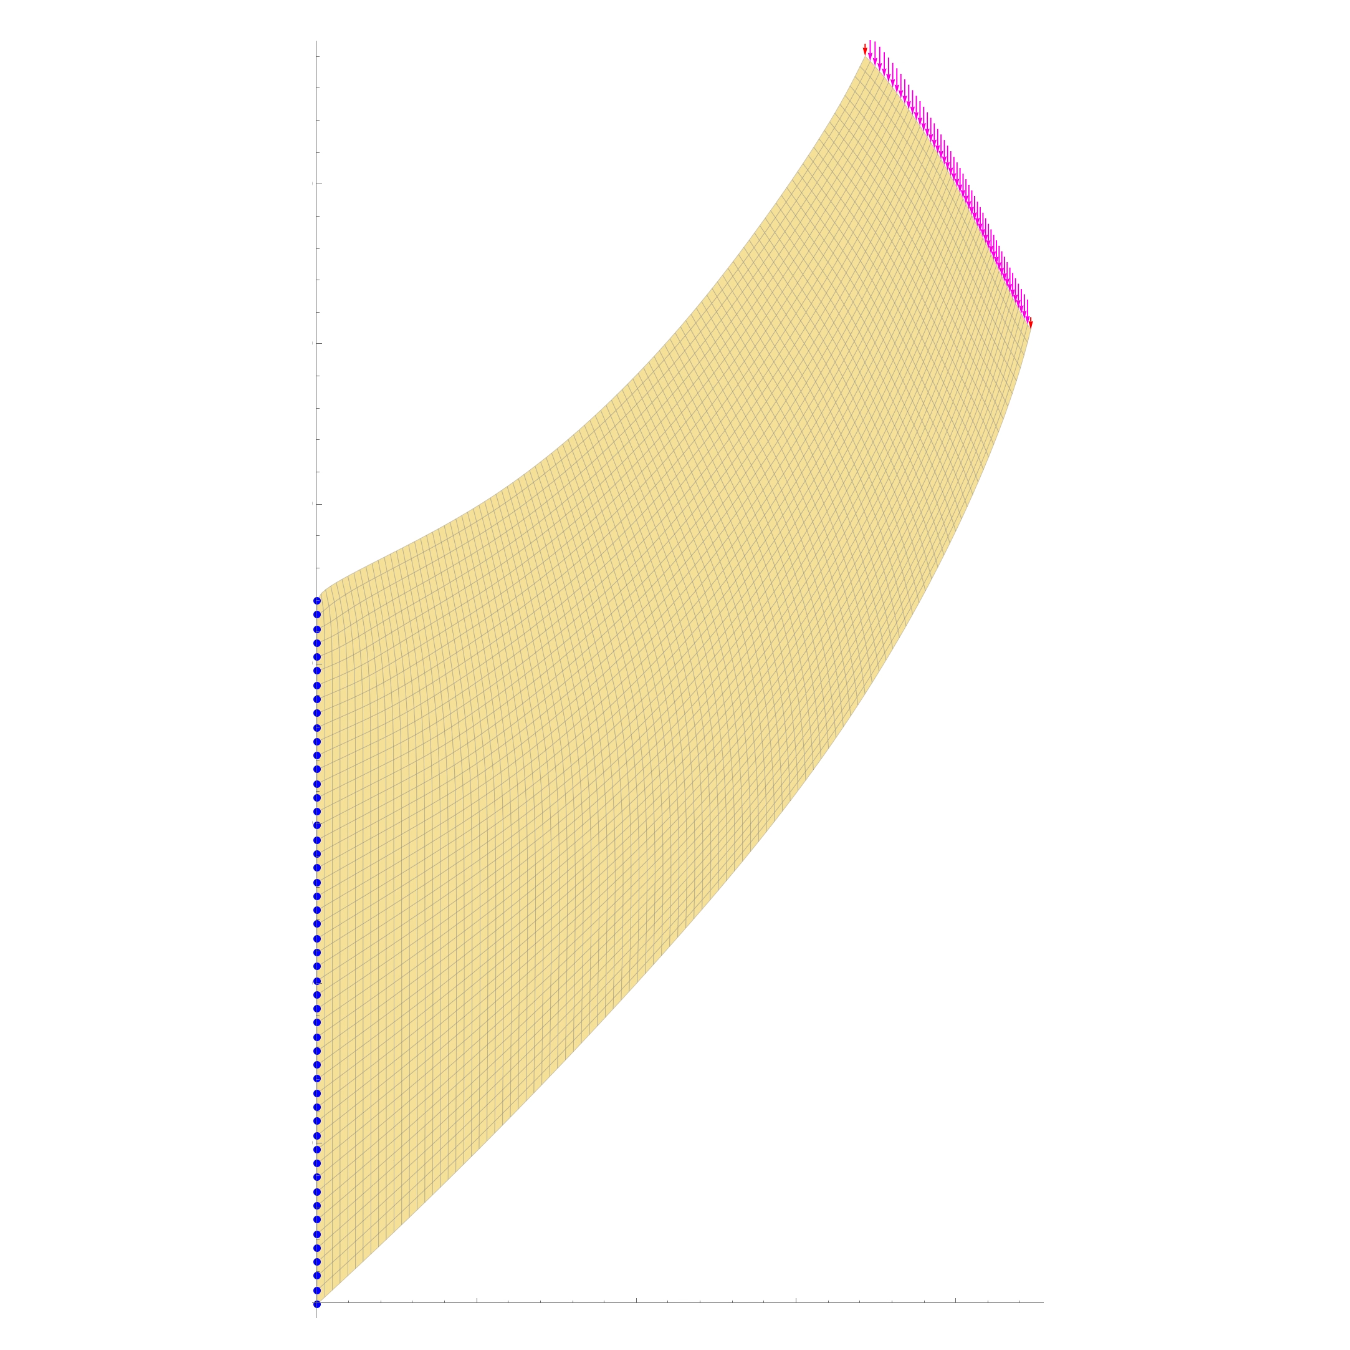
\includegraphics[width=0.3\linewidth]{iso3.png}\hfill
			\end{minipage}\hfill
			\begin{minipage}{0.5\linewidth}
				\centering
	\fontsize{4pt}{4pt}\selectfont{kinematic hardening\\}
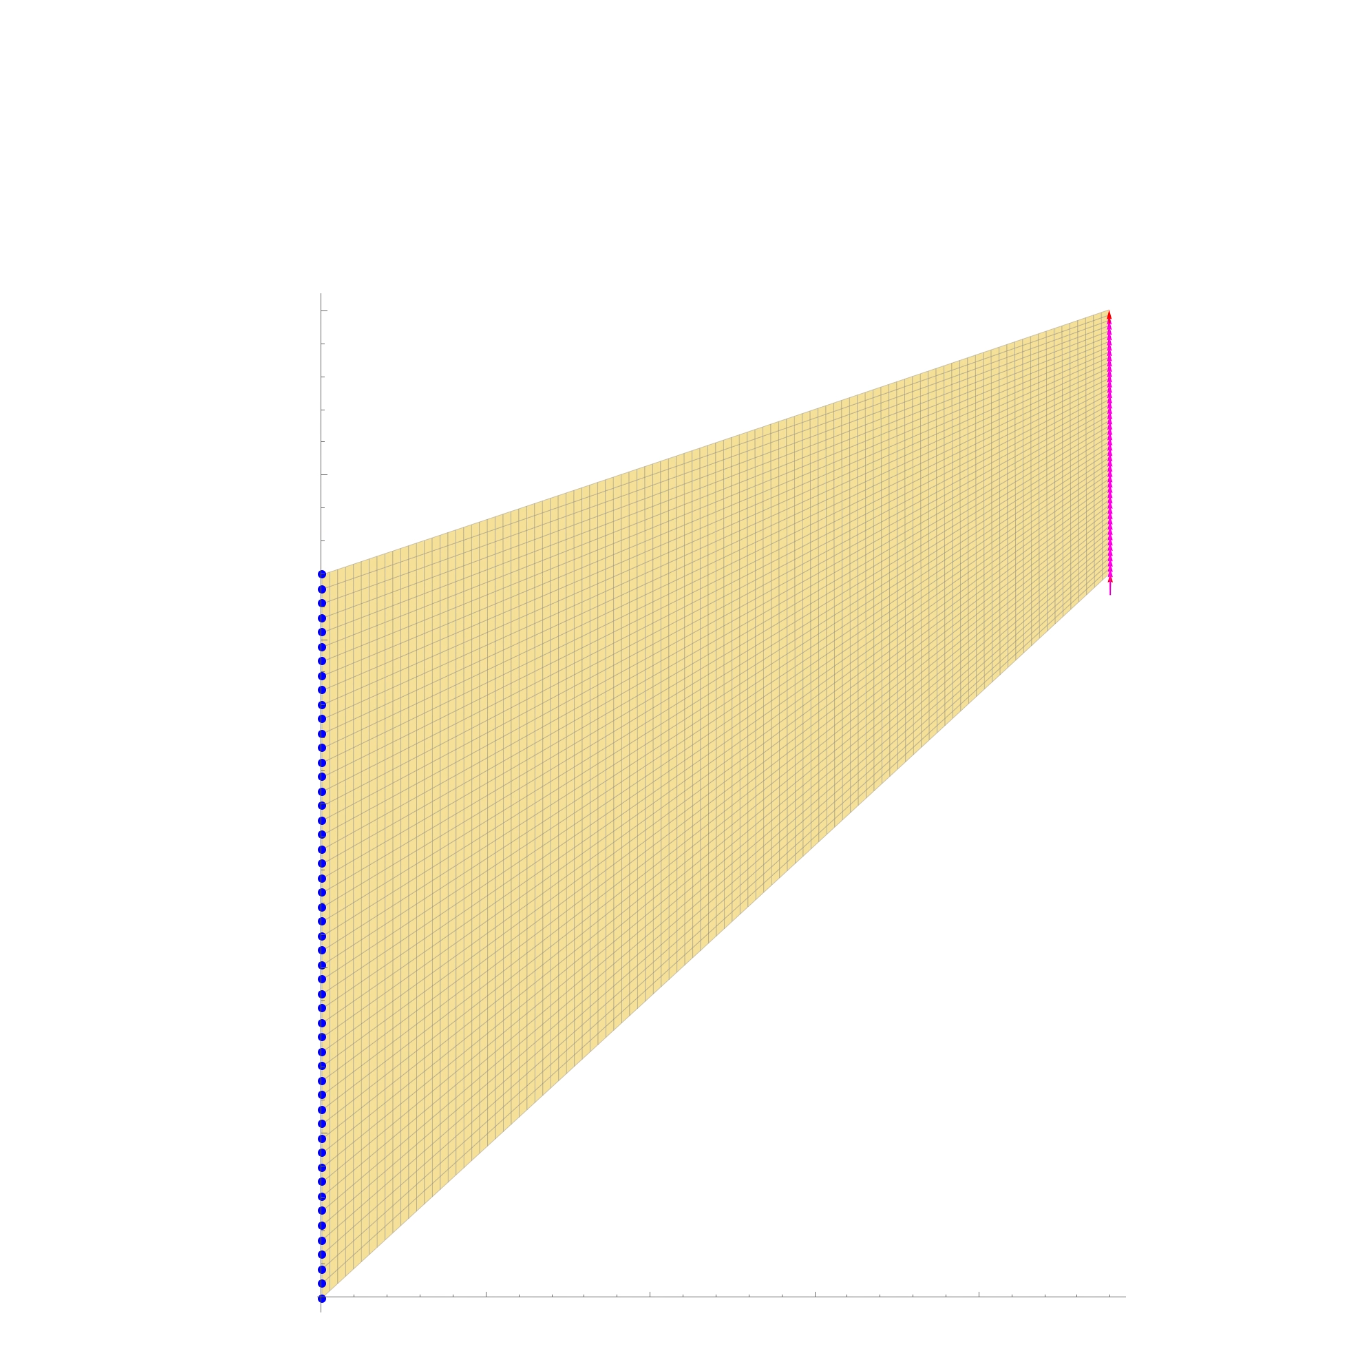
\includegraphics[width=0.3\linewidth]{kin1.png}\hfill
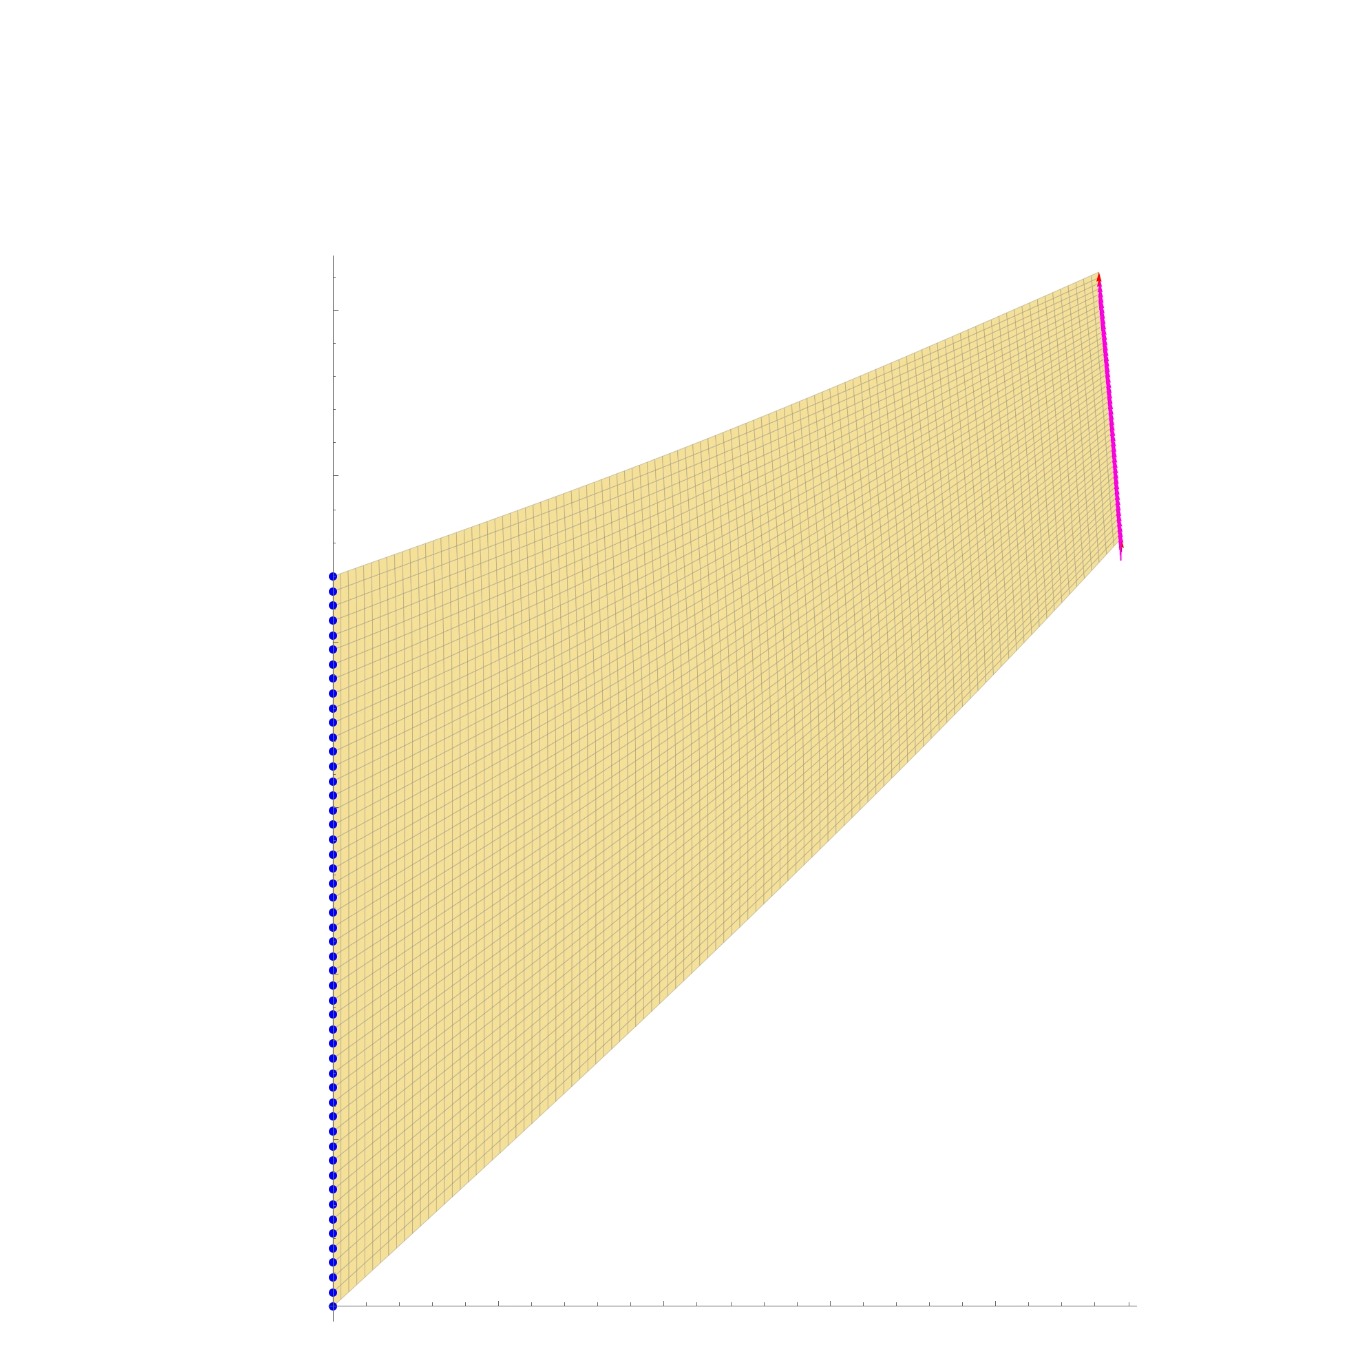
\includegraphics[width=0.3\linewidth]{kin2.png}\hfill
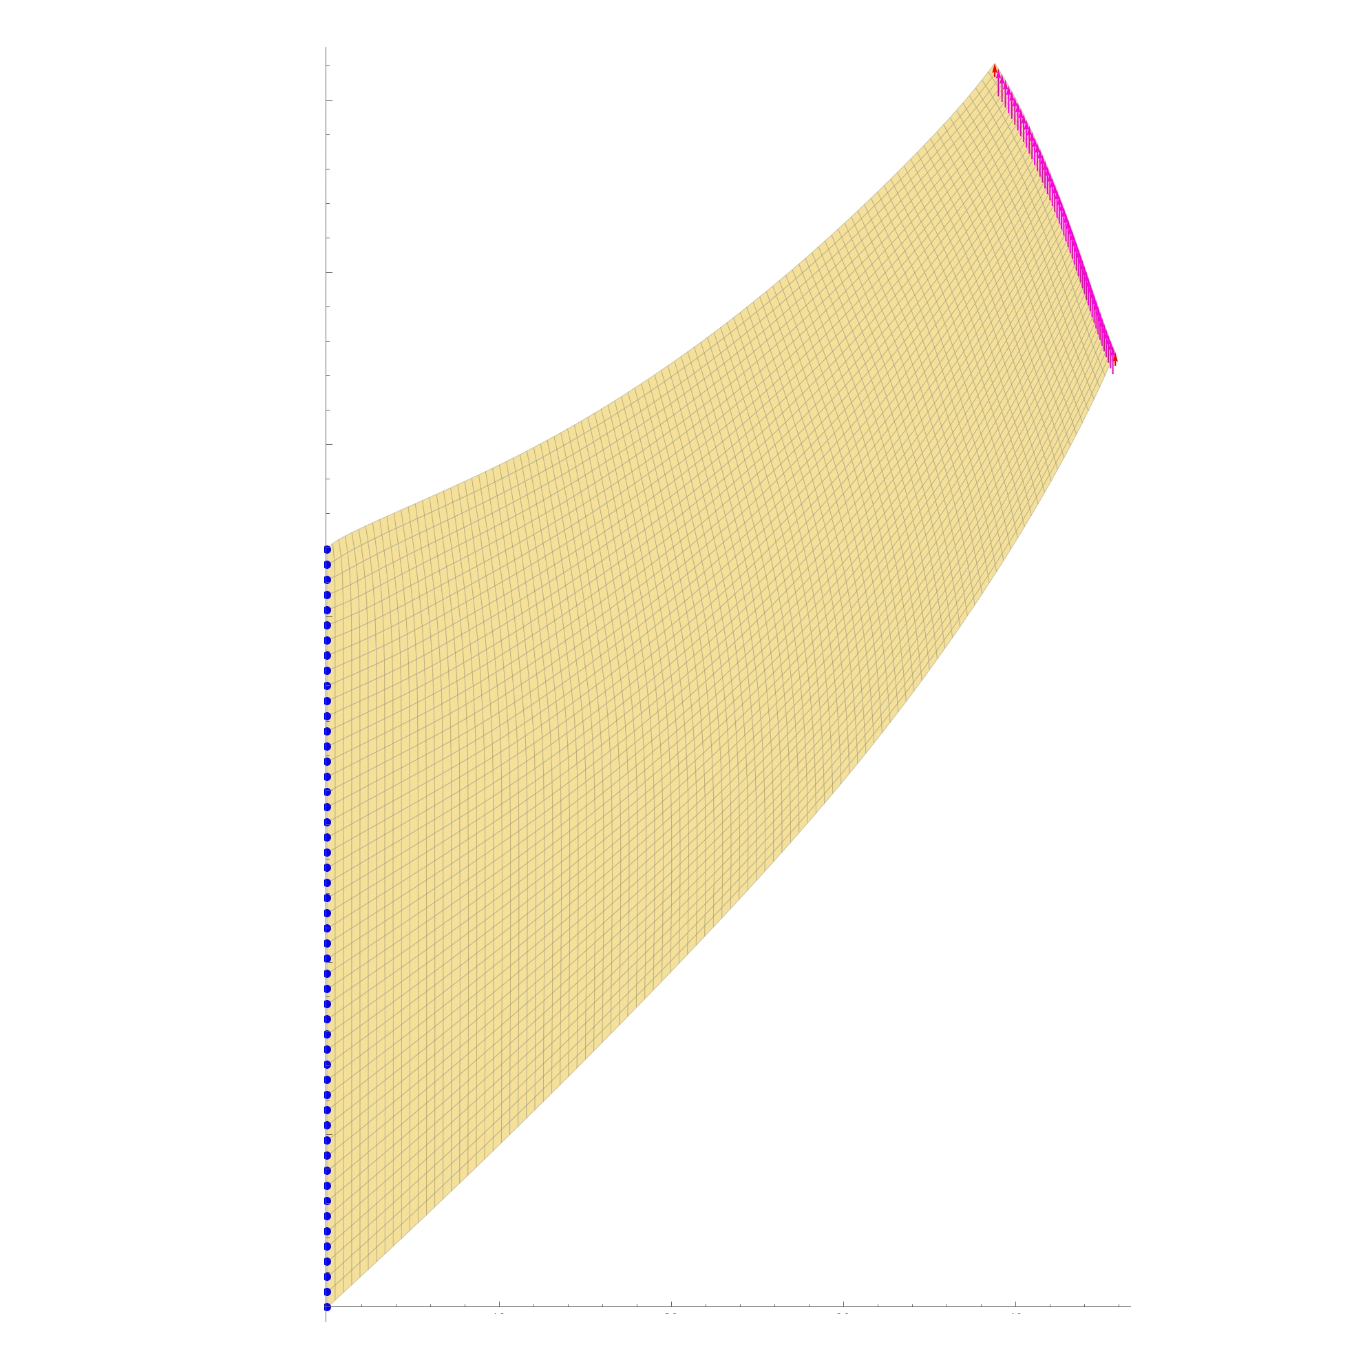
\includegraphics[width=0.3\linewidth]{kin3.png}\hfill
			\end{minipage}\hfill
		\begin{minipage}{0.5\linewidth}
			\centering
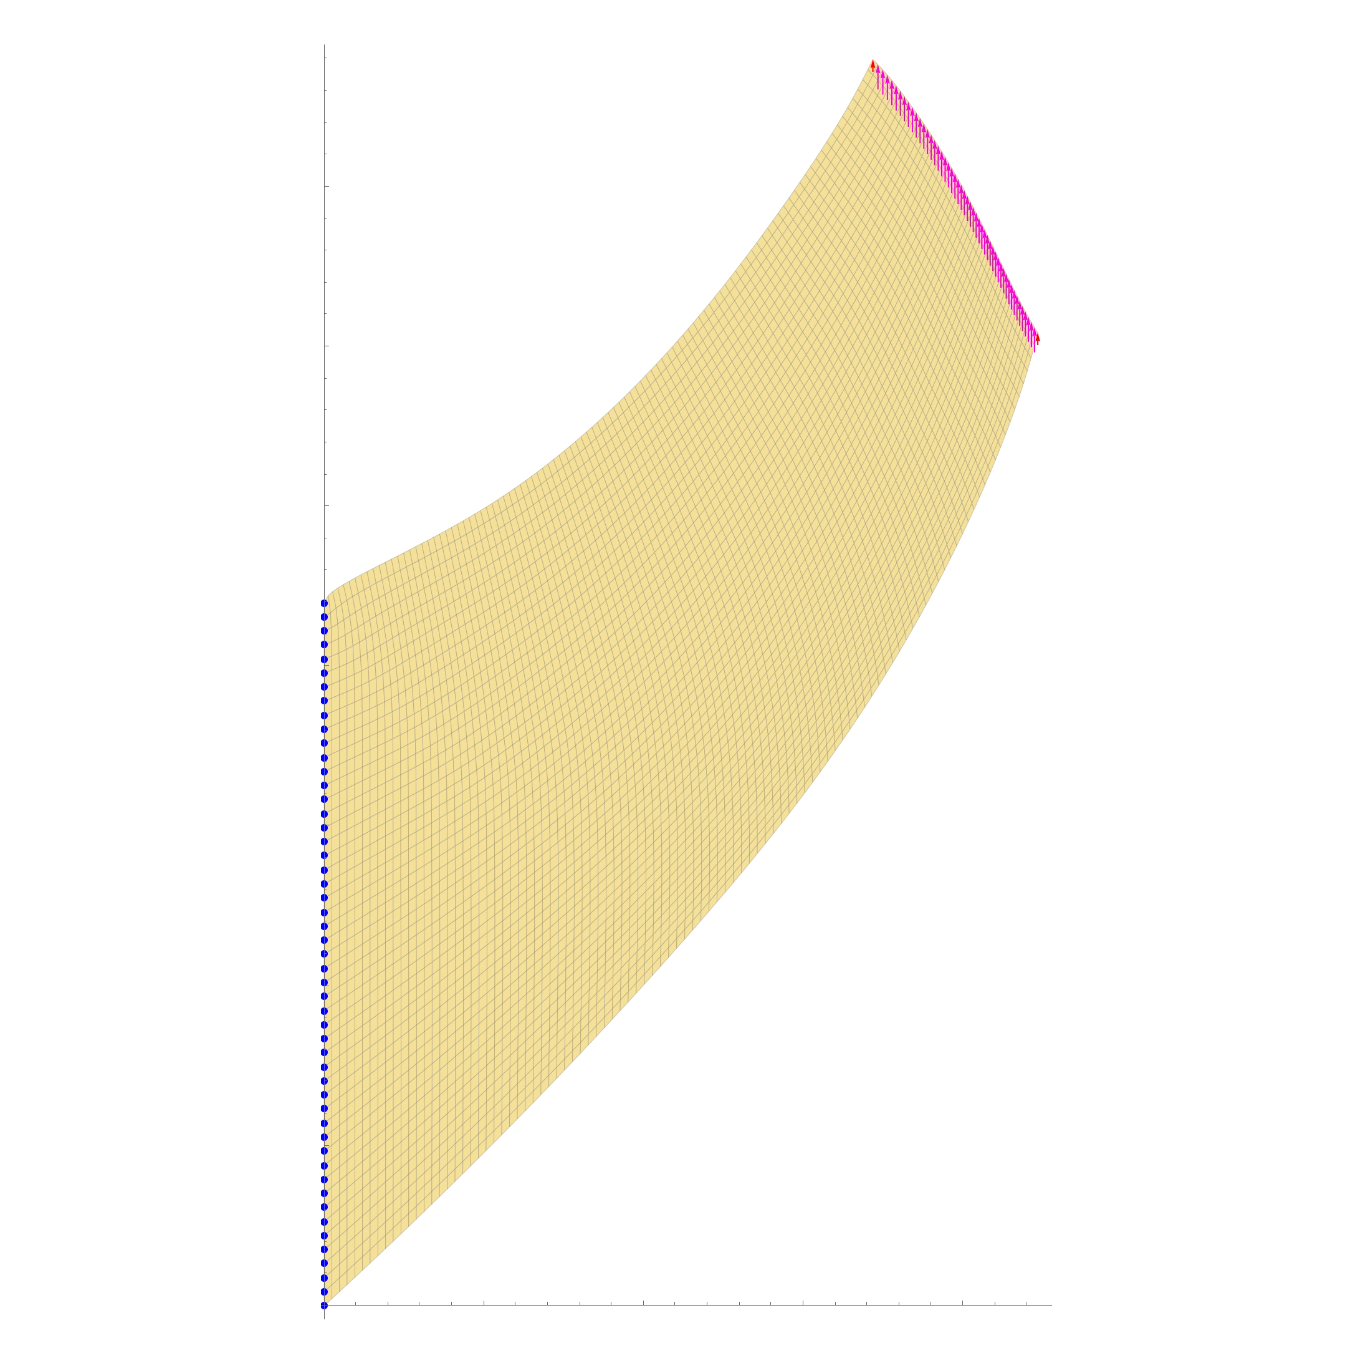
\includegraphics[width=0.3\linewidth]{iso4.png}\hfill
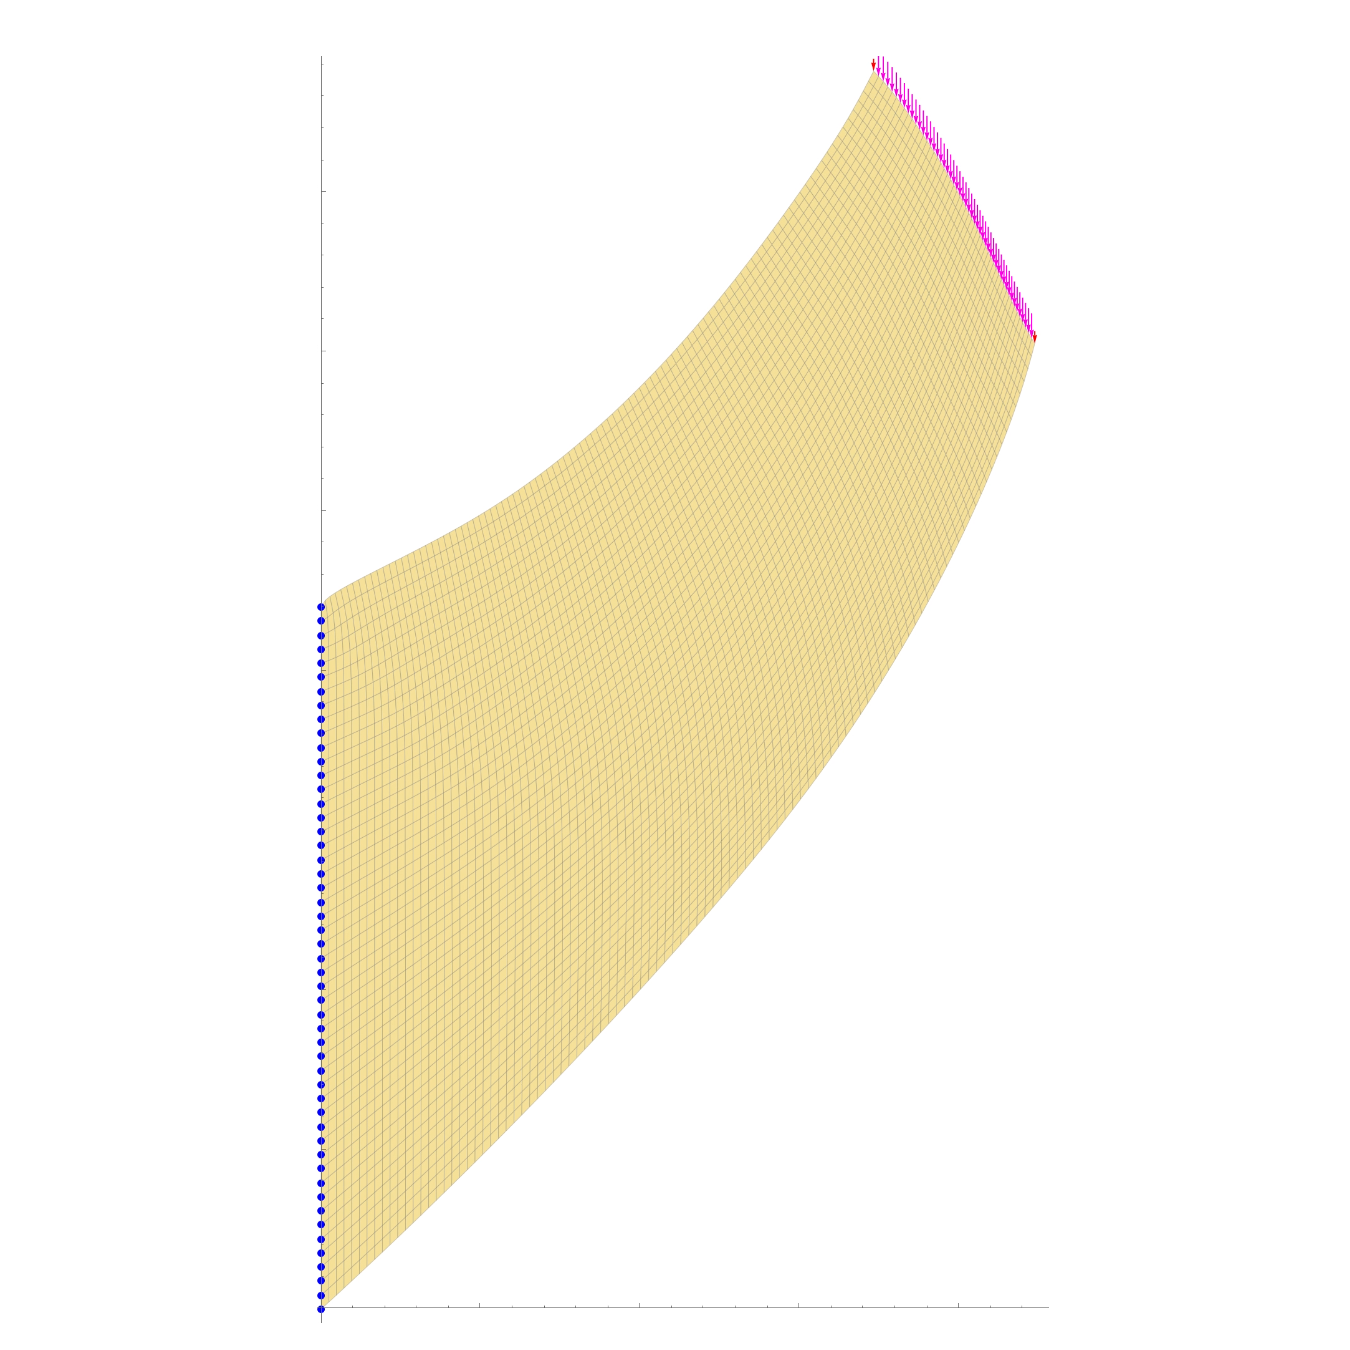
\includegraphics[width=0.3\linewidth]{iso5.png}\hfill
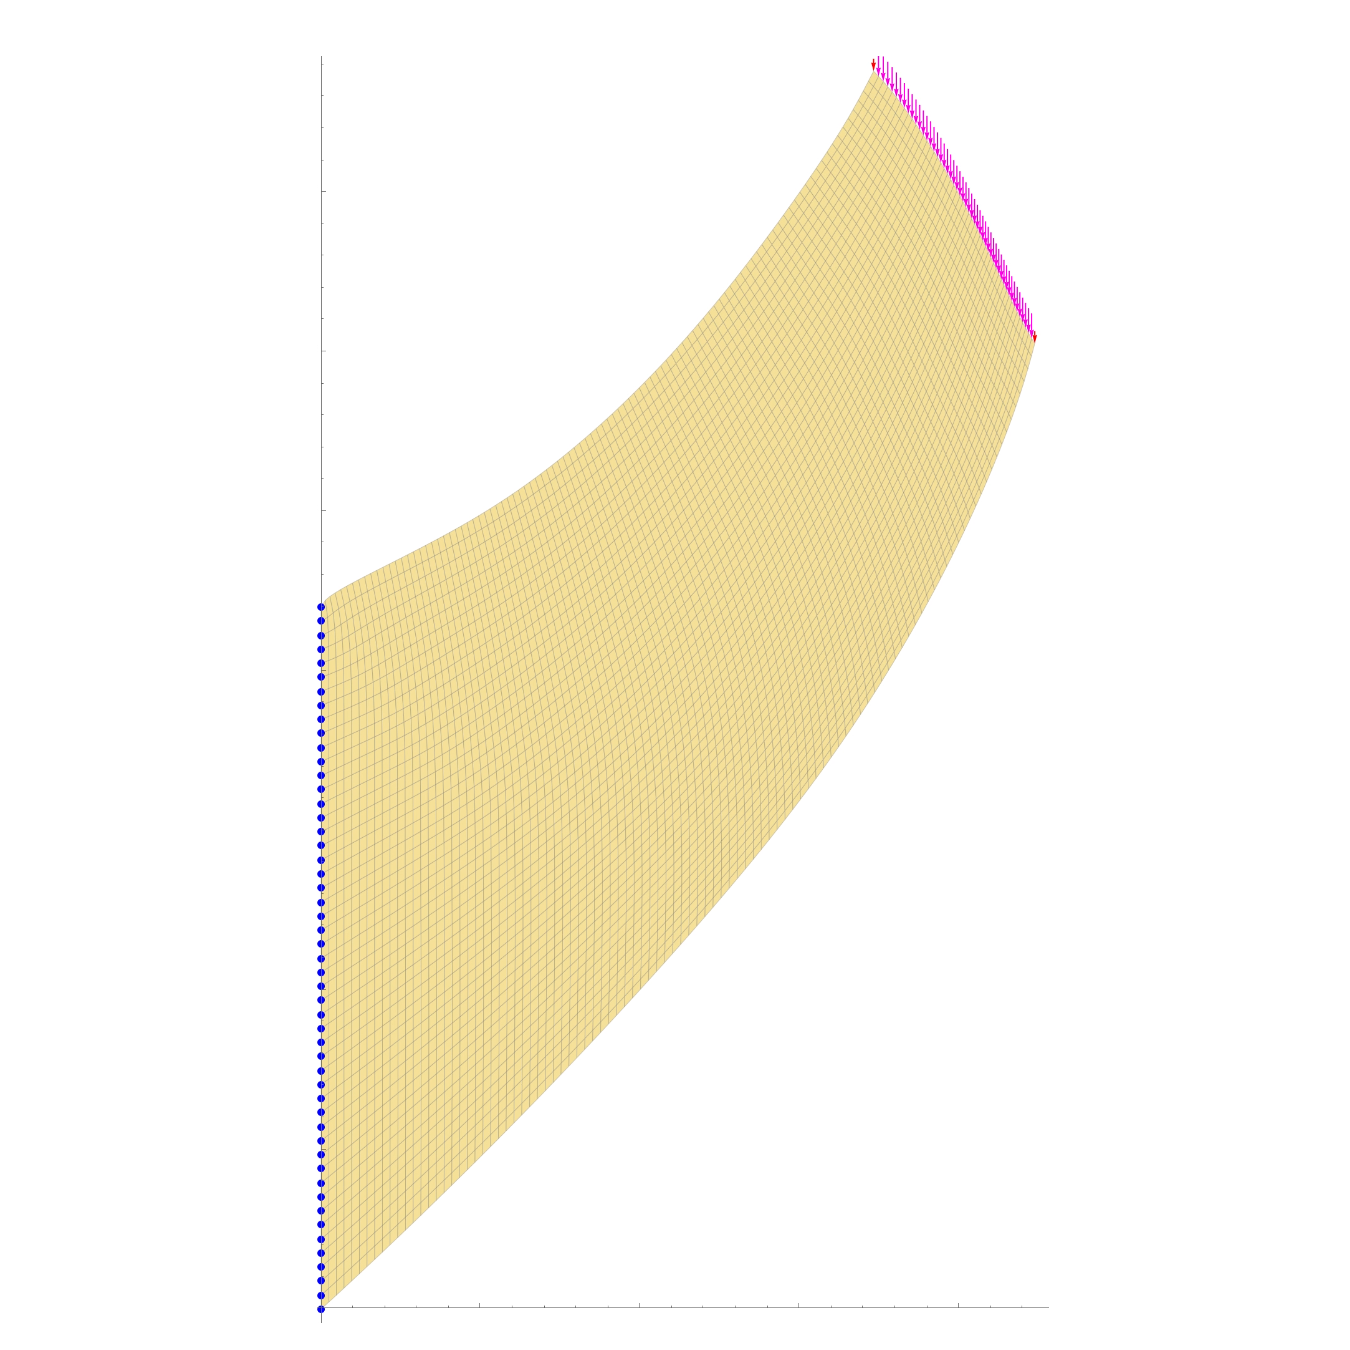
\includegraphics[width=0.3\linewidth]{iso6.png}\hfill
		\end{minipage}\hfill
		\begin{minipage}{0.5\linewidth}
			\centering
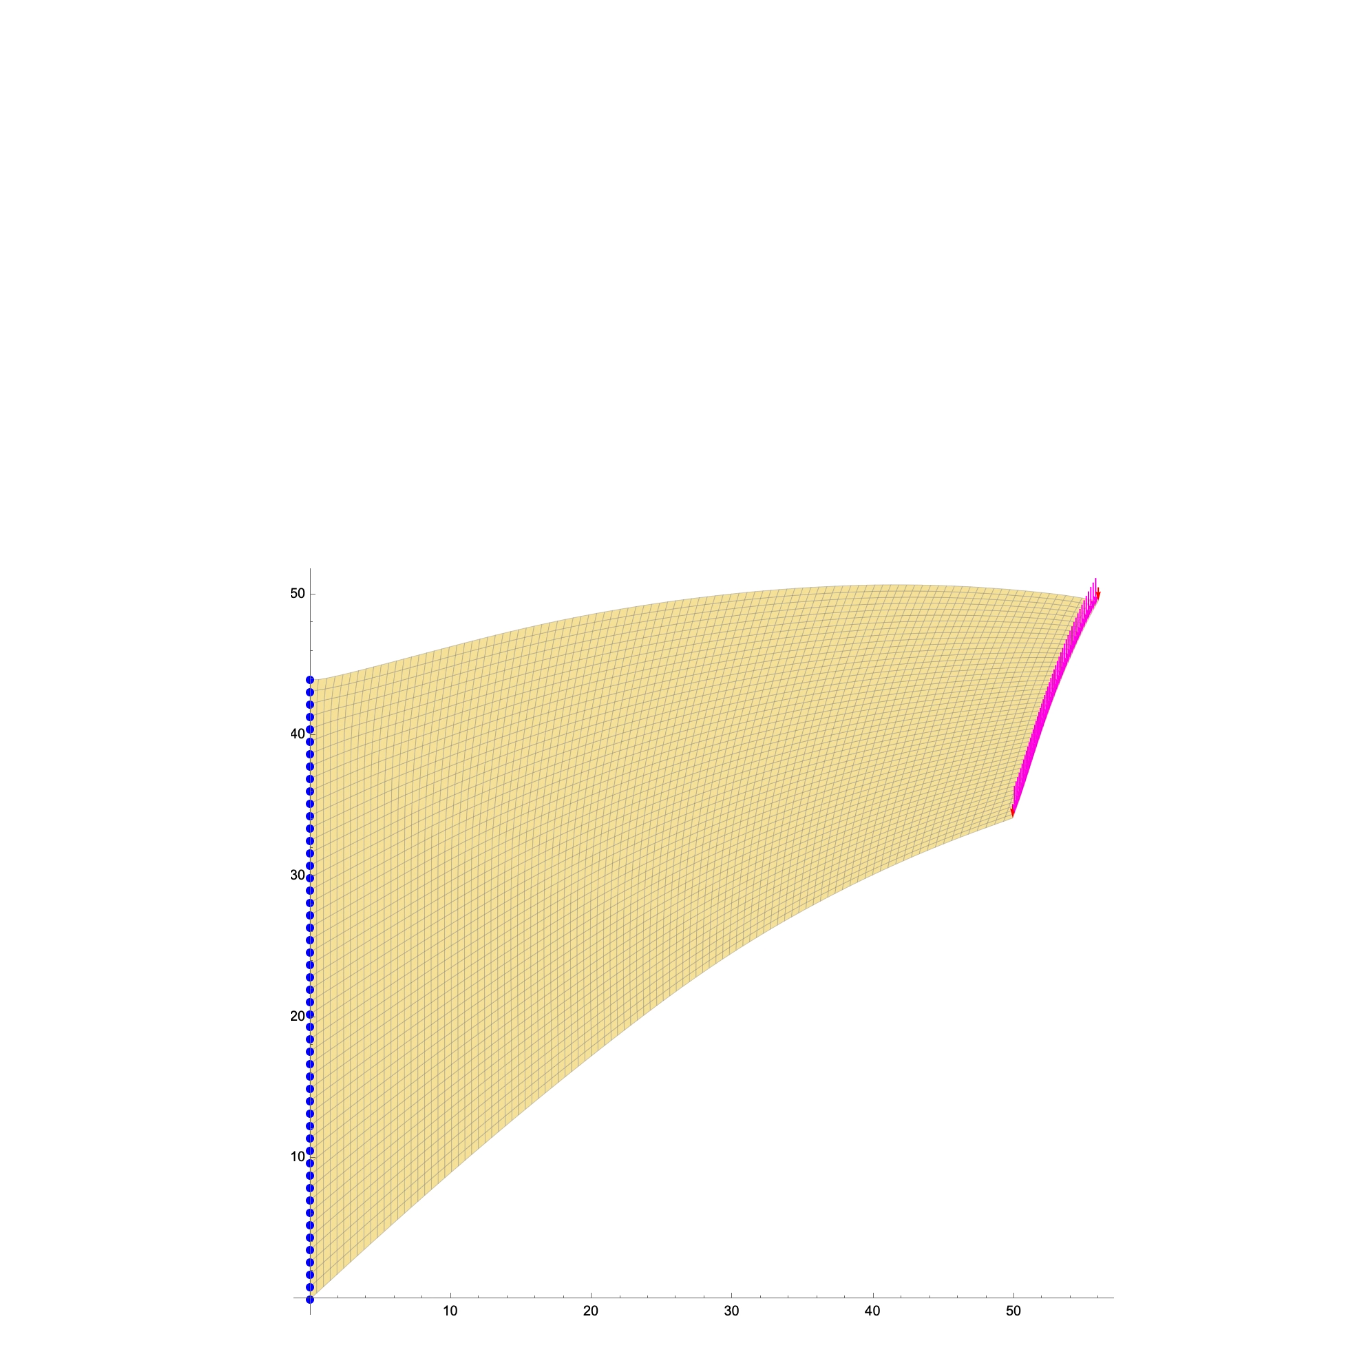
\includegraphics[width=0.3\linewidth]{kin4.png}\hfill
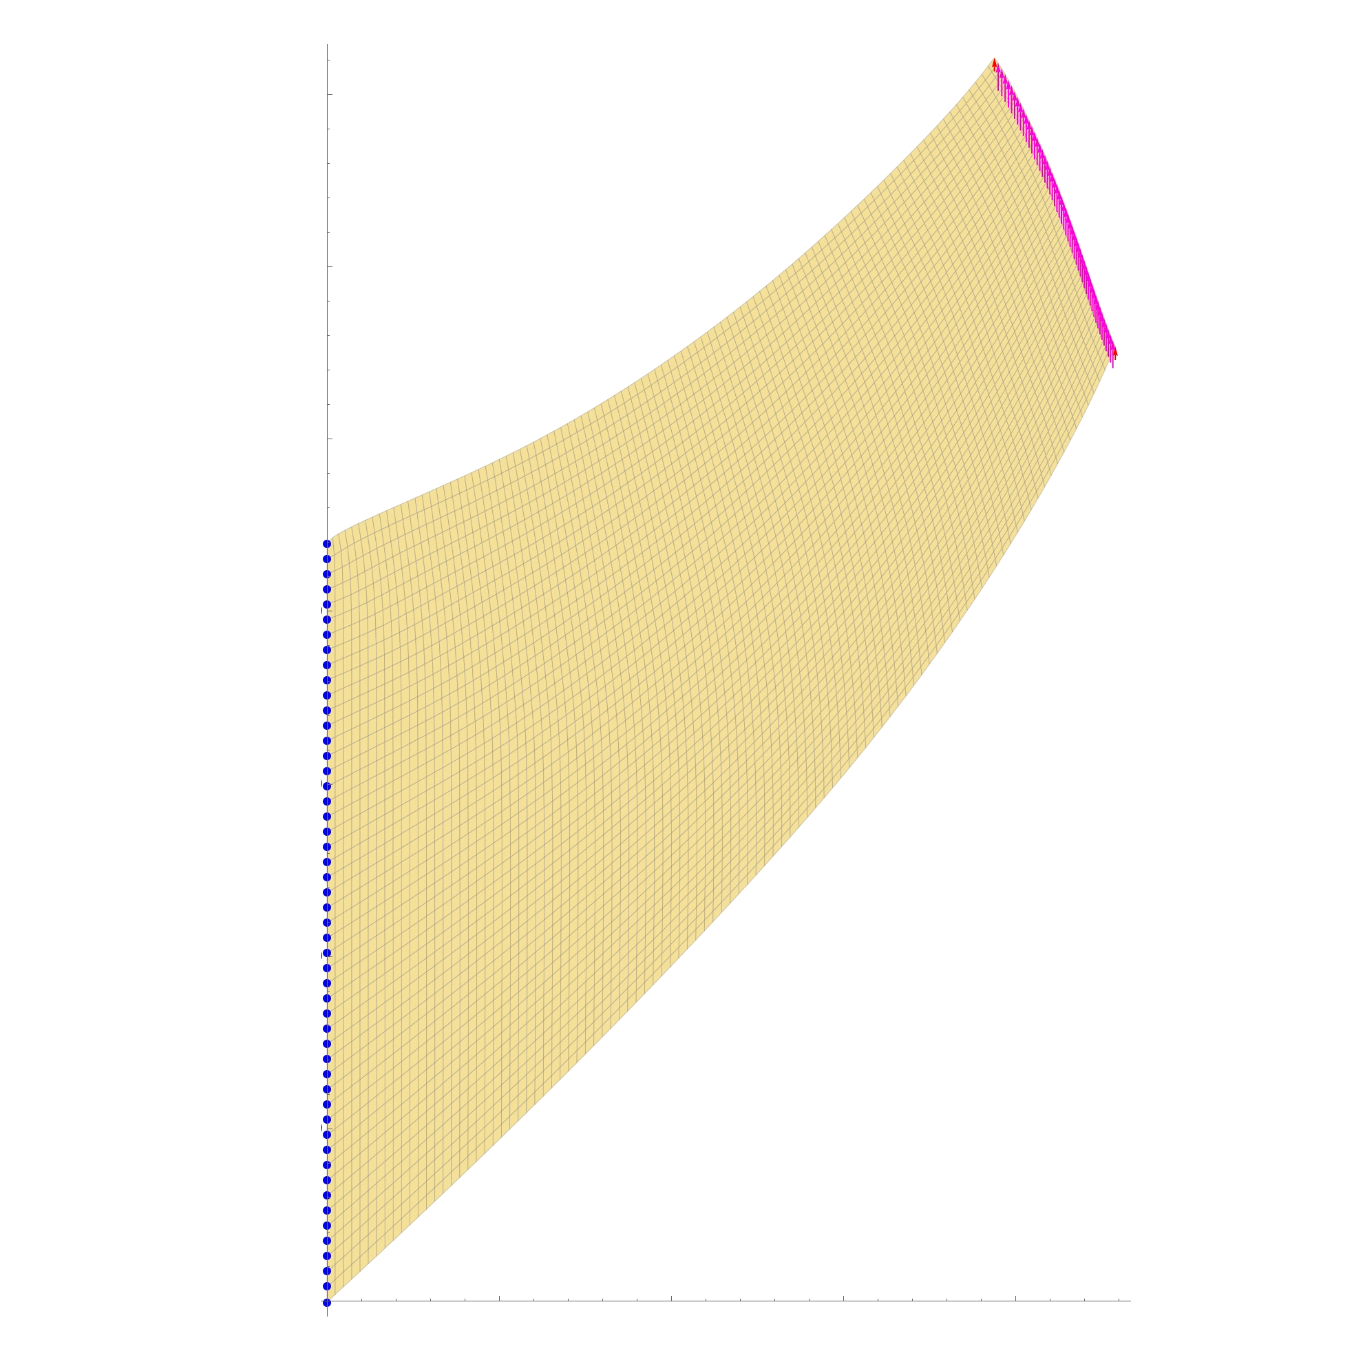
\includegraphics[width=0.3\linewidth]{kin5.png}\hfill
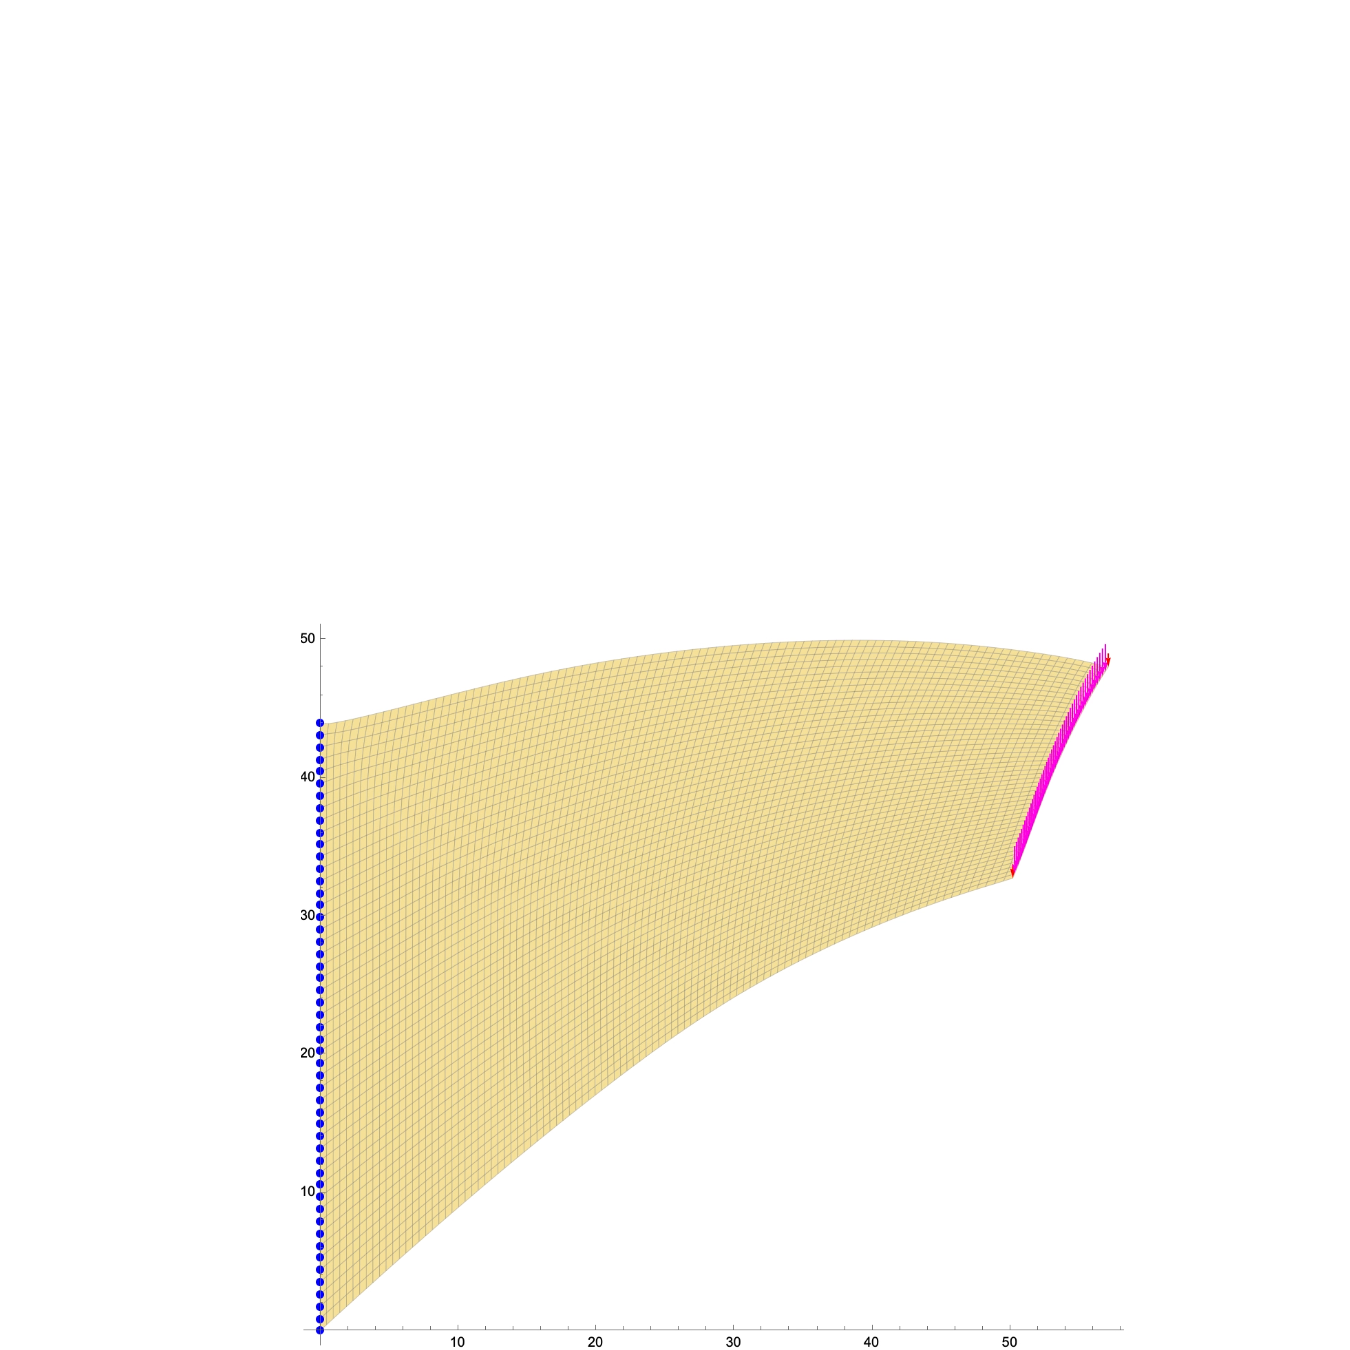
\includegraphics[width=0.3\linewidth]{kin6.png}\hfill
		\end{minipage}\hfill
		\end{minipage}\hfill
		%%%%%%%%%%%%%%%%%
	\end{figure}
\end{frame}

\end{document}